%!TEX root = principal.tex
A palavra automação vem do latim \emph{automatus} -- mover por si mesmo. Logo a automação de uma tarefa consiste em fazer com que tal tarefa seja realizada de modo autônomo, sem envolver trabalho humano. Isto pode ser por diversos motivos: seja por que é uma tarefa perigosa e portanto queremos aumentar a segurança das pessoas, como num processo que envolva alta temperatura, por exemplo; seja para fazer a tarefa de forma mais rápida, seja para melhorar a qualidade do produto final ou seja porque simplesmente o custo do trabalho humano é muito elevado. Logo, podemos definir automação da seguinte forma:
\begin{quote}
  Automação é a substituição do trabalho humano por sistemas autônomos visando melhorar segurança, qualidade, produção e custos.
\end{quote}

Neste contexto, automação industrial é nada mais que a automação de um sistema industrial, ou de um sistema de manufatura. Embora manufatura venha de fazer com as mãos, a revolução industrial mudou este conceito, passando a significar a fabricação de praticamente qualquer produto. Do ponto de vista econômico, a manufatura é a transformação de materiais (matéria prima) em itens de maior valor (produto). Isto é conseguido por uma determinada sequência de processos químicos e físicos. De forma mais sucinta:
\begin{quote}
	Manufatura é a transformação de matéria prima em produtos pela aplicação de um ou mais processos.
\end{quote}

Logo, a automação industrial consiste em fazer os processos necessários para a manufatura com o mínimo de esforço ou interferência humana, visando melhor segurança, qualidade, produção e custo. Note-se que por esforço humano, queremos dizer tanto esforço físico quanto mental, logo uma máquina bastante complexa mas que funcione a manivela, não se classificaria como automação; da mesma forma uma máquina que não exija esforço físico mas requer atenção constante também não é automatizada (seria apenas mecanizada).

\section{História}
É interessante pegar alguns pontos chaves na história da automação. Embora várias máquinas mecânicas de diversas graus de complexidade já existissem, como por exemplo relógios mecânicos desde o século VIII na china e desde o século XIII na Europa e os robôs de Pierre Jaquet-Droz, do século XVIII, considera-se que a revolução industrial iniciou com a invenção do tear mecânico por Cartwright em 1785, que realiza um movimento relativamente complexo de forma automática a partir de uma roda d'água.

Por volta de 1788 houve a invenção do mecanismo de regulagem de fluxo de vapor de James Watt, o que permitiu controlar a potência de caldeiras e outras máquinas a vapor, manipulando uma potência muito maior que uma roda d'água. Isto foi um grande impulso para a mecanização, mas a verdadeira automatização ainda ficava muito restrita devido a dificuldade de realizar processos complexos de forma automática. Ou seja, retirava-se grande parte do esforço físico do homem, mas ainda era necessário muito esforço mental.

Em 1820 o francês Charles Babbage, trabalhando para automatizar o processo mental do cálculo matemático, começou a desenvolver a sua máquina diferencial, que hoje chamaríamos de uma calculadora mecânica. Ela evoluiu até o conceito da máquina analítica, descrita em 1837, que é considerada o primeiro projeto de computador, embora apenas partes dela tenham sido efetivamente construídas.

 Em 1880, Herman Hollerith criou um novo método, baseado na utilização de cartões perfurados e calculadoras mecânicas, para automatizar algumas tarefas de tabulação do censo dos EUA que antes duravam 10 anos. Com seu método, o processo era concluído em 6.

Ao longo da primeira metade do século XX foram utilizados muitos sistemas eletromecânicos para o controle de processos industriais. Eram os chamados circuitos chaveados, que utilizavam relês para o controle lógico e para o comando de motores.

Em 1936, Alan Turing descreveu um \emph{computador universal} em seu artigo “On Computable Numbers, with an Application to the Entscheidungsproblem”, o que hoje é conhecido como uma \emph{Máquina de Turing}. Suas idéias foram desenvolvidas em 1944, com a construção do Colossus, considerado como o primeiro computador, embora tivesse a função específica de quebrar o código criptográfico alemão na segunda guerra. Ele consistia de um circuito com 1600 a 2400 válvulas com capacidade de processamento de vinte e cinco mil caracteres por segundo. A titulo de comparação, os computadores de casa de hoje em dia atingem 10 bilhões de cálculos por segundo.

O avanço da eletrônica fez que que a capacidade de processamento dos computadores aumentasse de forma exponencial. Atualmente o mais rápido computador do mundo é o chinês Sunway TaihuLight, que faz 93 quatrilhões de cálculos por segundo, consumindo 15 MW.

Na década de 60 a General Motors fez uma especificação de um CLP -- Controlador Lógico Programável, que é um computador voltado para o controle de processos industriais. Em 1968 foi criado o primeiro.

Hoje em dia toda automação está relacionada a sistemas computadorizados, seja em CLPs, CNCs, robôs industriais, automação dos sistemas de apoio a produção, entre outros.

\section{Classificação}

Hoje em dia se definem, grosso modo, 3 tipos de automação, tal qual mostra a figura \ref{fig:tipos_automacao}: fixa, flexível e programável.
\begin{figure}[hbt]
	\begin{center}
%		\includegraphics[width=0.6\textwidth]{tipos_automacao}
	\tikzstyle{area}=[draw,rectangle,rounded corners,text centered,text width=2.2cm,minimum height=1.2cm]
	\begin{tikzpicture}
		\draw[very thick, ->, >=stealth'](0,0)--(5.5,0);
		\draw(5.5,0)node[below left]{Diversidade};
		\draw[very thick, ->, >=stealth'](0,0)--(0,3.3);
		\draw(0,3.3)node[above left, rotate=90]{Quantidade};
		\draw(1.25,2.5)node[area]{Fixa} (2.5,1.55)node[area]{Flexível} (4,0.6)node[area]{Programável};
	\end{tikzpicture}
	\end{center}
	\caption{Tipos de automação industrial quanto a quantidade e diversidade de produtos.}
	\label{fig:tipos_automacao}
\end{figure}

A automação fixa é aplicada à produção de um único produto (ou com mínimas variações), em grandes quantidades: refinaria de petróleo, parafuso, tampas de garrafa, clips, biscoito, cerveja, etc. Ela utiliza equipamentos feitos sob medida para cada processo, que portanto tem alto custo inicial mas grande produtividade.

A automação flexível é aplicada à produção de produtos parecidos, em que pequenas modificações permitem a alteração do produto, como por exemplo mudança de um perfil a ser prensado ou extrudado ou a mudança das quantidades do mesmo conjunto de matérias primas (mudança de receita). Tipicamente é feita a chamada fabricação em lotes, onde entre um lote e outro se alteram as peças e/ou as sequências a serem seguidas de forma automática para ter o menor tempo parado possível. Exemplos são livros, circuitos integrados, potes de plástico, máquinas de café.

A automação programável é para produção de produtos diferentes mas cujo volume de produção não justifica um processo único. Ela usa máquinas de propósito geral, tais como robôs, ferramentas de controle numérico e impressoras 3d, onde a definição do processo é quase toda feita por \emph{software}, de modo que o custo do maquinário é diluído em diversos produtos.

A tendência é cada vez mais ter a automação flexível e programável aumentando a capacidade de produção, de modo que a flexível vai ocupando nichos da fixa e a programável da flexível. Apesar disso, em vários casos é difícil imaginar alguns produtos deixando de utilizar a automação fixa.

\section{Pirâmide de automação}

A automação em larga escala de uma grande indústria envolve muito mais que a mera manufatura e inclui problemas de abastecimento, armazenagem, análise de mercado, exigências ambientais, entre várias outras coisas. Uma forma de se separar os diferentes problemas da automação é através da chamada Pirâmide de Automação, mostrada na figura \ref{fig:piramide}.

\begin{figure}[htb]
	\begin{center}
\begin{tikzpicture}[y=0.80pt, x=0.8pt,xscale=0.4,yscale=-0.4, inner sep=0pt, outer sep=0pt]
    \path[fill=black] (530,582.41803) node[above right] (text3018)
      {Instrumentação};
    \path[fill=black] (530,511.83002) node[above right] (text3022) {Controle};
    \path[fill=black] (530,441.0715) node[above right] (text3794)
      {Supervisão};
    \path[fill=black] (530,370.13507) node[above right] (text3798) {Gerência
      de manufatura};
    \path[fill=black] (530,299.51303) node[above right] (text3804)
      {Planejamento estratégico};
      \path[cm={{1.01932,0.0,0.0,1.01932,(-6.1462,-4.25386)}},draw=black,fill=c00ffff,miter
        limit=4.00,line width=2pt] (320.0000,252.3622) -- (423.9230,432.3622) --
        (527.8461,612.3622) -- (320.0000,612.3622) -- (112.1539,612.3622) --
        (216.0770,432.3622) -- cycle;
      \path[cm={{0.80176,0.0,0.0,0.79778,(63.47204,51.63306)}},draw=black,fill=c00ff00,miter
        limit=4.00,line width=2pt] (320.0000,252.3622) -- (423.9230,432.3622) --
        (527.8461,612.3622) -- (320.0000,612.3622) -- (112.1539,612.3622) --
        (216.0770,432.3622) -- cycle;
      \path[cm={{0.60132,0.0,0.0,0.59833,(127.61319,101.96534)}},draw=black,fill=cffff00,miter
        limit=4.00,line width=2pt] (320.0000,252.3622) -- (423.9230,432.3622) --
        (527.8461,612.3622) -- (320.0000,612.3622) -- (112.1539,612.3622) --
        (216.0770,432.3622) -- cycle;
      \path[cm={{0.40088,0.0,0.0,0.39889,(191.75434,152.29762)}},draw=black,fill=cff6600,miter
        limit=4.00,line width=2pt] (320.0000,252.3622) -- (423.9230,432.3622) --
        (527.8461,612.3622) -- (320.0000,612.3622) -- (112.1539,612.3622) --
        (216.0770,432.3622) -- cycle;
      \path[cm={{0.20044,0.0,0.0,0.19944,(255.8955,202.62989)}},draw=black,fill=cff5555,miter
        limit=4.00,line width=2pt] (320.0000,252.3622) -- (423.9230,432.3622) --
        (527.8461,612.3622) -- (320.0000,612.3622) -- (112.1539,612.3622) --
        (216.0770,432.3622) -- cycle;
    \begin{scope}[shift={(3.29592,0)}]
      \path[fill=black] (309.04346,582.41803) node[above right] (text3824) {0};
      \path[fill=black] (310.00049,511.8302) node[above right] (text3828) {1};
      \path[fill=black] (309.28271,441.0715) node[above right] (text3832) {2};
      \path[fill=black] (309.00244,370.13507) node[above right] (text3836) {3};
      \path[fill=black] (309.45361,299.51303) node[above right] (text3840) {4};
    \end{scope}
    \path[fill=black] (79.834969,582.41803) node[above left] (text3858) {Sensores
      eatuadores};
    \path[fill=black] (79.875984,511.8302) node[above left] (text3862) {CLP, SDCD,
      CNC};
    \path[fill=black] (81.256844,441.0715) node[above left] (text3866) {SCADA,
      HMI};
    \path[fill=black] (80.245125,370.13507) node[above left] (text3870) {PIMS, MES,
      LIMS, WMS};
    \path[fill=black] (79.999031,299.51303) node[above left] (text3874) {ERP};

\end{tikzpicture}
	\end{center}
	\caption{Pirâmide de automação.}
	\label{fig:piramide}
\end{figure}

Note que esta não é a única representação da pirâmide: umas começam pelo 1, outras tem apenas 4 camadas, e assim por diante, logo mais importante que o número de cada camada é o que tais camadas significam.

\begin{description}
	\item[Nível 0: Instrumentação] Camada onde se encontram instrumentos, sensores, motores,
máquinas, etc. Consistem nos equipamentos do chamado ``\emph{chão de fábrica}''.
\item[Nível 1: Controle] Controle automático da planta -- onde se localizam os Controladores
Lógico-Programáveis (CLP), os Sistemas Digitais de Controle Distribuído (SDCD), os Controles Numéricos Computadorizados (CNC) e/ou computadores de controle.
\item[Nível 2: Supervisão] Supervisão e controle do processo através de Interfaces Homem-Má
quina (IHMs) ou SCADA (\emph{Supervisory Control And Data Acquisition}).
\item[Nível 3: Gerenciamento da Manufatura] Gestão dos recursos da planta e controle da produção.  Sistemas PIMS
(\emph{Process Information Management System}) e MES (\emph{Manufacturing Execution Systems}).
\item[Nível 4: Planejamento Estratégico] Gestão dos recursos e produção da empresa como um todo. ERP –
\emph{Enterprise Resources Planning}.
\end{description}

A figura \ref{fig:automacao} mostra um diagrama em blocos de um processo automatizado, contendo os blocos representativos dos níveis 0 até o 3 da pirâmide de automação. A instrumentação consiste de sensores para acompanhar as variáveis controladas de um processo e atuadores para alterar as variáveis manipuladas. Como tais atuadores irão operar é definido pelo controle, em função de parâmetros definidos pelo supervisório. Este também monitora estas informações e as repassa ao sistema de gerenciamento, que aglutina dados de diversos processos para a tomada de decisões de mais alto nível.
\begin{figure}[htb]
	\begin{center}
    \includegraphics[width=0.7\textwidth]{figuras/automacao}
	\end{center}
	\caption{Diagrama em blocos da automação de um processo.}
	\label{fig:automacao}
\end{figure}

Este texto faz um estudo da automação industrial de modo \emph{bottom-up}: começando do nível 0 até o nível 3. O nível 4 é mais importante para um estudo de engenharia de processo ou de produção e portanto não será abordado.
